
Typical software applications for language processing consist of several components that mirror different aspects of language and of the task they implement. Figure \ref{fig:textprocessingarch_en} displays a highly simplified architecture that can be found in a text processing system. The first three modules deal with the structure and meaning of the text input:

\begin{enumerate}
\item Pre-processing: cleaning up the data, removing formatting, detecting the input language, detecting if the text lacks diacritics, etc.
\item Grammatical analysis: finding the verb and its objects, reflexive pronouns, etc.;  detecting the sentence structure.
\item Semantic analysis: disambiguation (Which meaning of \emph{mier} is the right one in a given context?), resolving anaphora and referring expressions like \emph{on}, \emph{to auto}, etc.; representing the meaning of the sentence in a machine-readable way
\end{enumerate}

Task-specific modules then perform many different operations such as
automatic summarisation of an input text, database look-ups and many
others. At the figure \ref{fig:textprocessingarch_en}, we will
illustrate core application areas and highlight their core modules.
Again, the architectures of the applications are highly simplified and
idealised, to illustrate the complexity of Language Technology
applications in a generally understandable way.

After introducing the core application areas, we will give a short
overview of the situation in language technology research and education,
concluding with an overview of past and ongoing research programs. At
the end of this section, we will present an expert estimation on the
situation regarding core language technology tools and resources on a
number of dimensions such as availability, maturity, or quality. This
table gives a good overview on the situation of language technology for
Slovak.

\begin{figure*}[ht]
  \colorrule{grey3}{\textwidth}{1.5pt}
  \center
  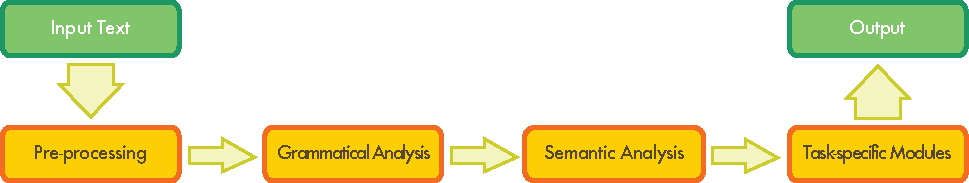
\includegraphics[width=\textwidth]{../_media/english/text_processing_app_architecture}
  \caption{A typical text processing architecture}
  \label{fig:textprocessingarch_en}
  \colorrule{grey3}{\textwidth}{1.5pt}
\end{figure*}

